\documentclass{beamer}
\usetheme[secheader]{Boadilla}
\usepackage[utf8]{inputenc}
\usepackage[czech]{babel}
\usepackage{hyperref}
\hypersetup{
unicode=true,}

\mode<presentation>
{

\title{Konečné automaty}
\author{Kateřina Fořtová (xforto00)}

\AtBeginSubsection[]
{
  \begin{frame}<beamer>{Outline}
    \tableofcontents[currentsection,currentsubsection]
  \end{frame}
}

\begin{document}

\begin{frame}
  \titlepage
\end{frame}

\begin{frame}{Konečné automaty}
  \begin{itemize}
  \item {Teoretický výpočetní model používaný v~informatice pro~studium formálních jazyků}
  \end{itemize}
  \pause
  \begin{alertblock}{Definice}
  \begin{itemize}
   \item{Definován jako uspořádaná pětice ($S$,$\Sigma$,$\sigma$, $s$, $A$), kde $S$ je konečná neprázdná množina stavů, $\Sigma$ je neprázdná množina vstupních symbolu (\textit{abeceda}), $\sigma$ je přechodová funkce, co popisuje pravidla přechodů mezi stavy, $s$ je počáteční stav, $s$ $\in$ $S$, $A$ je množina příjímacích stavů ($A$ $\subset$ $S$)}
  \end{itemize}
  \end{alertblock}
\end{frame}

\begin{frame}{Grafické znázornění konečného automatu}
  \begin{columns}
    \column{5cm}
      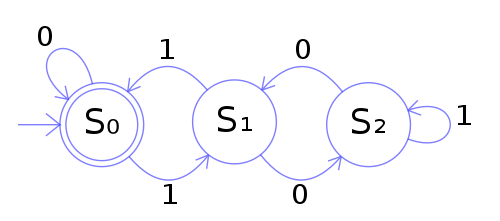
\includegraphics[width=5cm]{znazorneni.png}
    \column{5cm}
      \begin{itemize}
        \item{Kolečka znázorňují jednotlivé stavy a šipky mezi nimi popisují jednotlivé přechody}
      \end{itemize}
  \end{columns}
\end{frame}

\begin{frame}{Znázornění konečného automatu ve formě tabulky}
  \begin{columns}
    \column{5cm}
      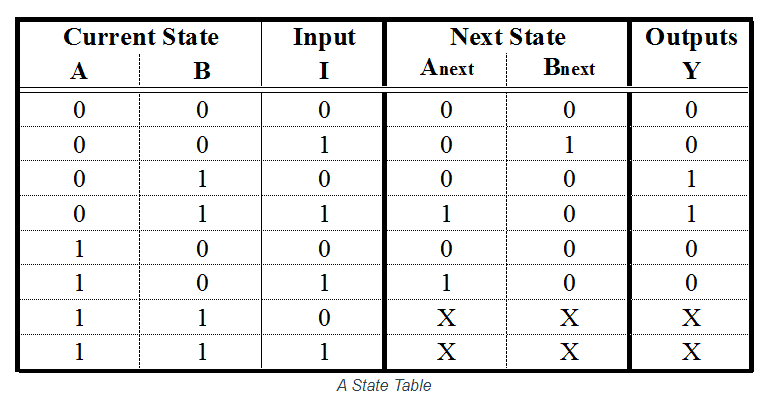
\includegraphics[width=5cm]{statetable.PNG}
    \column{5cm}
      \begin{itemize}
        \item{Řádky znázorňují stavy a přechody a sloupce písmena}
      \end{itemize}
  \end{columns}
\end{frame}

\begin{frame}{Znázornění konečného automatu ve~formě stavového stromu}
  \begin{columns}
    \column{5cm}
      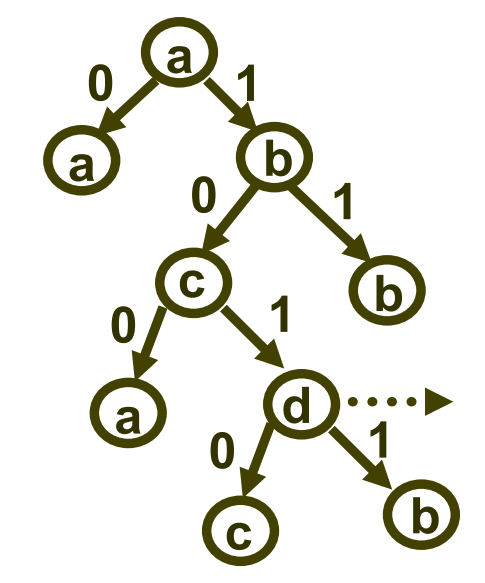
\includegraphics[width=5cm]{tree.PNG}
    \column{5cm}
      \begin{itemize}
        \item{Vrcholy znázorňují stavy a hrany přechody}
        \item{Znázorňují se pouze dosažitelné stavy}
      \end{itemize}
  \end{columns}
\end{frame}

\begin{frame}{Dělení konečných automatů}
  \begin{itemize}
  \item{determistické -- má pouze jeden počáteční stav a přechodová funkce vrací jeden stav}
  \pause
  \item{nedetermistické -- nejednoznačný, může mít více počátečních stavů a přechodová funkce vrací množinu stavů}
  \end{itemize}
\end{frame}


\begin{frame}{Funkce konečného automatu}
  \begin{itemize}
  \item{automat se nachází v~počátečním stavu}
  \item{automatu je předložen konečný vstupní řetězec postavený nad~jeho vstupní abecedou}
  \item{automat přečte a odebere symbol ze~vstupního řetězce}
  \item{automat provede přechod na~základě tohoto symbolu a aktuálního vnitřního stavu (je-li definován)}
  \item{druhý až čtvrtý bod se opakuje tak dlouho, dokud není celý vstupní řetězec přečten}
  \end{itemize}
\end{frame}

\begin{frame}{Konečné automaty typu Mealy}
  \begin{columns}
    \column{5cm}
      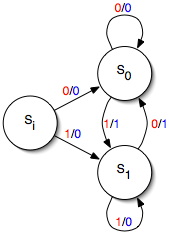
\includegraphics[width=5cm]{mealy.png}
    \column{5cm}
      \begin{itemize}
        \item{Zobecnění typu Moore}
        \item{Výstup nezávisí pouze na~vnitřním stavu, ale i na~vstupu}
        \item{Do~výstupní funkce vstupuje i jako parametr aktuální prvek vstupní abecedy}
      \end{itemize}
  \end{columns}
\end{frame}

\begin{frame}{Konečné automaty typu Moore}
  \begin{columns}
    \column{5cm}
      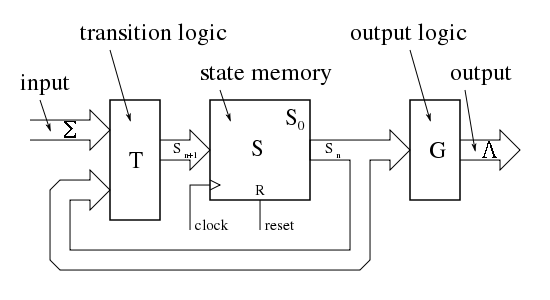
\includegraphics[width=5cm]{moore.png}
    \column{5cm}
      \begin{itemize}
        \item{Končený počet vnitřních stavů}
        \item{Každý vnitřní stav má definovanou právě jednu hodnotu na~výstupu}
        \item{Definovaný vnitřní stav, ve kterém se nachází před~zadáním prvního vstupního symbolu a pravidla pro~přechody mezi jednotlivými stavy}
      \end{itemize}
  \end{columns}
\end{frame}

\begin{frame}{Zdroje}
  \begin{itemize}
  \item\href{https://ktiml.mff.cuni.cz/~bartak/automaty/lectures/lecture01.pdf}{Roman Barták -- Automaty a gramatiky}
  \item\href{http://voho.eu/wiki/konecny-automat/}{voho.eu -- Konečný automat}
  \item\href{https://en.wikipedia.org/wiki/Finite-state_machine}{en.wikipedia.org -- Finite-state machine}
  \item\href{http://lucie.zolta.cz/index.php/statnice-vsb/9-skola-vsb/zaklady-teoreticke-informatiky/4-konecne-automaty}{Lucie Žoltá -- Konečné automaty}
  \end{itemize}
\end{frame}

\end{document} }
